
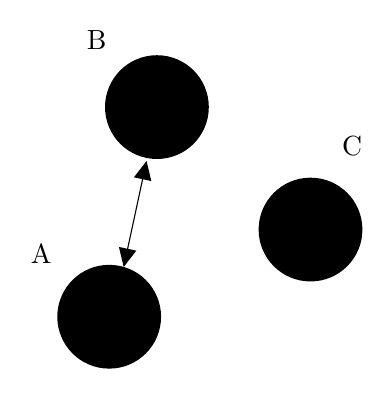
\begin{tikzpicture}[x=0.75pt,y=0.75pt,yscale=-1,xscale=1]
%uncomment if require: \path (0,300); %set diagram left start at 0, and has height of 300

%Shape: Circle [id:dp1418814839562289] 
\draw  [draw opacity=0][fill={rgb, 255:red, 0; green, 0; blue, 0 }  ,fill opacity=1 ] (116,196) .. controls (116,182.19) and (127.19,171) .. (141,171) .. controls (154.81,171) and (166,182.19) .. (166,196) .. controls (166,209.81) and (154.81,221) .. (141,221) .. controls (127.19,221) and (116,209.81) .. (116,196) -- cycle ;
%Shape: Circle [id:dp3981484481701938] 
\draw  [draw opacity=0][fill={rgb, 255:red, 0; green, 0; blue, 0 }  ,fill opacity=1 ] (139,95) .. controls (139,81.19) and (150.19,70) .. (164,70) .. controls (177.81,70) and (189,81.19) .. (189,95) .. controls (189,108.81) and (177.81,120) .. (164,120) .. controls (150.19,120) and (139,108.81) .. (139,95) -- cycle ;
%Shape: Circle [id:dp7390139799048381] 
\draw  [draw opacity=0][fill={rgb, 255:red, 0; green, 0; blue, 0 }  ,fill opacity=1 ] (213,154) .. controls (213,140.19) and (224.19,129) .. (238,129) .. controls (251.81,129) and (263,140.19) .. (263,154) .. controls (263,167.81) and (251.81,179) .. (238,179) .. controls (224.19,179) and (213,167.81) .. (213,154) -- cycle ;
%Straight Lines [id:da4506323249212101] 
\draw    (158.37,123.93) -- (148.63,169.07) ;
\draw [shift={(148,172)}, rotate = 282.17] [fill={rgb, 255:red, 0; green, 0; blue, 0 }  ][line width=0.08]  [draw opacity=0] (8.93,-4.29) -- (0,0) -- (8.93,4.29) -- cycle    ;
\draw [shift={(159,121)}, rotate = 102.17] [fill={rgb, 255:red, 0; green, 0; blue, 0 }  ][line width=0.08]  [draw opacity=0] (8.93,-4.29) -- (0,0) -- (8.93,4.29) -- cycle    ;

% Text Node
\draw (102,160) node [anchor=north west][inner sep=0.75pt]   [align=left] {A};
% Text Node
\draw (129,57) node [anchor=north west][inner sep=0.75pt]   [align=left] {B};
% Text Node
\draw (252,108) node [anchor=north west][inner sep=0.75pt]   [align=left] {C};


\end{tikzpicture}